\chapter{Middleend} \label{middleend}


Middleend je napsán v jazyce Typescript pro Node.js za pomoci
RESTful frameworku Restify.
Ekosystém Node.js byl zvolen kvůli své škálovatelnosti a
rychlosti vývoje. Typescript, který je transpilován do JavaScriptu,
pak pomáhá omezit problémy spojené se slabě typovaným JavaScriptem
a přináší funkce v JavaScriptu nepřítomné nebo které by se
v JavaScriptu musely implementovat ručně či náročně.
Restify slouží jako užitečná abstrakce nad Node.js API.

Po spuštění se serverovému objektu Restify předají funkce pro parsování
příchozích žádostí, CORS mezivsrstva (z angl. Cross-Origin Resource Sharing).
Zmíněné funkce jsou přímo z frameworku Restify a přidružených NPM knihoven.
Před nasazením hlavního routeru je ještě přidána vlastní vrstva, která ověřuje
klientův \uv{session token}, o kterém si povíme v podsekci o autentifikaci.

Hlavní router skládá dohromady všechny endpointy, které mohou být umístěny
přímo na hlavní router, nebo mohou být součástí podřadných routerů.
Jeden takový podřadný router má na starosti přihlašování.
Je samozřejmě možné dávat endpointy přímo na serverový objekt,
ale tím bychom se zbavili jisté flexibility, a nemohli tak snadno
určit kořenovou cestu pro všechny endpointy.
Zároveň si každý router může určit, jakou relativní cestu budou mít
routery podřadné.

Veškerá komunikace s klinty je ve formátu JSON.

\section{Konfigurace}

Paramatry pro Middleend lze nastavit ze dvou míst. Z konfiguračního souboru,
jenž se nachází ve složce \verb|/config| a stanovením proměnné prostředí
(angl. Environment Variable) s názvem \verb|NODE_CONFIG|, jejíž hodnoty
mají prioritu nad konfiguračním souborem. Formát konfigurace je JSON:

\begin{code}
{
    "db": {
        ...
    },
    "server": {
        "port": 8000,
        ...
        "sessionTokenExpiresInMillis": 86400000,
        "rootPath": ""
    },
    "_desc": "Local development config."
}
\end{code}

Middleend používá dva Postgres účty. První (cesta \verb|db.middleend|) je určen například pro
ověřování a změnu hesel. Druhý (cesta \verb|db.qdb|) zajišťuje žádosti na endpoint \verb|/qdb|.
Druhý účet má práva pouze na pohledy na tabulky v db a jeho
permise dále omezují permise konkrétního uživatele. Objekty v polích \verb|db.*| mají
položky \verb|host|, \verb|port|, \verb|user|, \verb|password|, \verb|database|, \verb|max|.
Všechna kromě \verb|max| jsou na první pohled srozumitelná. \verb|Max| určuje nejvyšší možný počet klientů v poolu.

Chceme-li například změnit port aplikace, nastavíme \verb|NODE_CONFIG|
na řetězec \uv{\{"server": 9000\}}. Při spouštění v produkci je 
nutné nastavit \verb|NODE_ENV| na \newline \uv{production}.

\begin{table} \centering
\begin{tabular}{ l l l }
    {\textbf{Cesta}} & {\textbf{Typ}} & {\textbf{Popis}} \\
    \hline
    server.port & int & Port serveru \\
    server.origins & [string] & Povolené zdroje žádostí \\
    server.logRequests & bool & Logování obsahu žádostí \\
    server.sessionSecret & string & Tvorba klíčů pro session token \\
    server.sessionTokenExpiresInMillis & int & Doba platnosti session tokenu \\
    server.rootPath & string & Cesta hlavního routeru \\
    \hline
    server.authentication.password & boolean & Povolení přihlášení heslem \\
    server.authentication.reader & boolean & Povolení přihlášení kartou \\
\end{tabular}
\caption{Seznam všech používaných hodnot kromě databázového připojení}
\label{tb03:configKeys}
\end{table}

\section{Autentifikace}

Autentifikace může probíhat různými způsoby. Po úspěšné autentifikaci
uživatele nebo například čtečky, obdrží klient \uv{session token}, který
použije pro další žádosti. Posílá se v HTTP hlavičce \verb|Authorization|
ve formátu \uv{Token <hodnota>}. Klient také obdrží jeho dobu platnosti
v milisekundách od času autentifikace. Důvod pro autentifikaci hlavičkou
místo běžných cookies je, že tak jednoduše zabráníme XSS (angl. Cross-site scriping).

Session token má následující podobu: \newline
\verb|<iv>.<tělo>.<timestamp vytvoření>.<hmac>|. \verb|Iv| je inicializační vektor \citep[viz][]{TechopediaIV}.
Algoritmus pro vytvoření byl převzán z
knihovny node-client-sessions společnosti Mozilla \citep[viz][]{MozillaSession}.
Funguje tak, že si vytvoříme klíč pro šifrování dat, která jsou ve formátu JSON,
a klíč pro podepsání konečné zprávy. Klíče vytvoříme z náhodného řetězce (\uv{session secret}) pomocí funkce HMAC.
Session secret musí zůstat tajný, jinak by si útočník mohl sám podepsat session tokeny.
Symetricky zašifrujeme data, přičemž přidáme inicializační vektor.
Poskládáme jednotlivé části dohromady a spočítáme z nich HMAC
(angl. Hash Message Authentication Code), jehož hodnotu přidáme na konec celého tokenu.
HMAC slouží jako ověření tokenu, pouze Middleend je schopen ji vytvořit \citep[viz][]{SecSA}.
Inicializační vektor, zašifrovaná data, HMAC hodnotu závěrečně zaenkódujeme do Base64 \citep[viz][]{RFC4649}.

Aby byl předložený session token platný, musí splňovat několik podmínek.
Nesmí být starý, tj. $t_v + t_e \geq t$,
kde $t$ je nynější čas, $t_v$ je čas vytvoření a $t_e$ je čas, za který se token stane neplatným.
Po dešifrování si spočítáme znovu HMAC, a ten se musí rovnat HMAC hodnotě z tokenu.
Poslední podmínkou je úspěšné parsování dešifrovaných JSON dat.

\subsection{Autentifikace heslem}

Pro solení a hashování hesel využívá Middleend algoritmus scrypt, který
je pro Node.js dostupný jako NPM balíček stejného jména \citep[viz][]{NodeScrypt}.
V porovnání s jinými kryptografickými algoritmy používanými pro zabezpečení hesel,
jako je pbkdf2 nebo bcrypt, má pár výhod.
Používá exponenciální čas a paměť, takže hardware optimalizovaný pro jeho výpočet
není natolik účinný, jako je hardware například pro pbkdf2 \citep[viz][]{MediumScrypt}.
V praxi je ale pbkdf2 s mnoha iteracemi účinný a používáný.

\begin{table}[htb]\centering
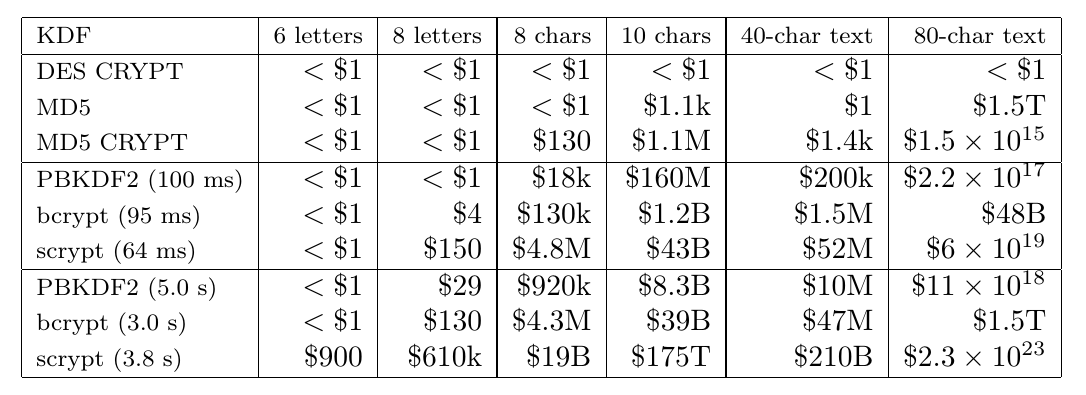
\includegraphics[width=140mm]{../img/crypto-funcs}
\textit{Časová hodnota v závorkách algoritmů určuje jejich náročnost.}
\caption{Odhadovaná cena hardwaru k prolomení hesla za 1 rok. \citep[viz][]{ScryptTable}}
\label{passwordCrackingCost}
\end{table}

Ceny hardwaru v tabulce~\ref{passwordCrackingCost} nebudou odpovídat dnešnímu stavu,
protože se výkon i cena hwardwaru od roku 2009, kdy byla tabulka vytvořena, změnily.
Každopádně je rozumné se domnívat, že crackování funkce scrypt je stále
nejdražší i dnes.

\section{Tunelování Postgresu pro Frontend}

Připojení k databázi je zprostředkováno NPM modulem \verb|pg| \citep[viz][]{NodePg}.
Ten umožňuje asynchronní přístup, předpřipravené žádosti a \uv{poolování}
(tj. máme \uv{pool} klientů, které si půjčujeme a vracíme je, jakmile je nepotřebujeme).

Jakmile je uživatel autentifikován platným session tokenem, je půjčen klient k databázi.
Dále se pošle databázi žádost, která zavolá backendovou funkci
\verb|session_user_set(user_id, secret)|, kde
\verb|user_id| je identifikátor uživatele a \verb|secret| je náhodný řetězec, který
potřebujeme pro odhlášení po spuštění uživatelského SQL.
Tím se určí uživatel a jeho permise.
Poté se spustí uživatelské SQL a odpověď se pošle uživateli.
Před posláním je ještě zpracována a některé části odpovědi z databáze jsou
vynechány, nebo přetransformovány.
V posledním kroku je uživatel odhlášen backendovou funkcí \verb|session_logout(secret)|,
kde \verb|secret| je náhodný řetězec, který jsme si vygenerovali při přihlášení.

\section{Transformace Postgres odpovědi}

Transformaci zajišťuje třída \verb|MiddleResponse|, která přijme původní odpověď databáze.
Odpověď databáze obsahuje proměnnou \verb|field| obsahující pole definic sloupců vrácených
z databáze.

\begin{code}
"fields": [
    {
        "name": "id",
        "tableID": 17249,
        "columnID": 1,
        "dataTypeID": 23,
        "dataTypeSize": 4,
        "dataTypeModifier": -1,
        "format": "text"
    },
    ...
]
\end{code}

V definici každého typu se chceme zbavit \verb|tableID|, \verb|columnID|, \verb|dataTypeID| a
nahradit je jmény, aby mohl Frontend data snadněji parsovat, čehož docílíme dotázáním se databáze.
Můžeme si všimnout, že v původní odpovědi už dostaneme název sloupce, jehož název může být
i agregační sloupec nebo sloupec přejmenovaný apod.
Dotazování z výkonostních důvodů provedeme při spuštění Middleendu.
SQL dotazy vypadají následovně:

\begin{code}
SELECT oid, typname FROM pg_type; -- id datových typů -> jména dt.
SELECT oid, relname FROM pg_class; -- id tabulek -> jména tabulek
\end{code}

Druhý SQL dotaz vrátí více než tabulky. Počet řádků je však dostatečně malý a nepotřebuje
moc paměťi navíc \citep[viz][]{PgType}, \citep[viz][]{PgClass}.

Odpovědi si uložíme do JavaScript objektu, který mapuje číselné identifikátory na řetězce.
JavaScript ale neumožňuje používat čísla jako klíče, tudíž si je převedeme při ukládání a
čtení na řetězec.

Konečná odpověď z Middleendu může vypadat následovně:

\begin{code}
{
    "rows": [
        [1, "Adam", "Warlock", "2014-04-08T22:00:00.000Z"],
        [2, "Harry", "Potter", "1990-07-31T22:00:00.000Z"]
    ],
    "rowCount": 2,
    "fields": [
        {
            "tableName": "wizards",
            "columnName": "id",
            "dataTypeName": "int4",
            "dataTypeSize": 4,
            "dataTypeModifier": -1,
            "format": "text"
        },
        ....
    ]
}
\end{code}
